for the PCB design, we followed multiples steps to ensure the design will be manufacturable, 
as well as correct in terms of signal integrity.

\section{PCB Requirements}
Before any layout step, we defined different specifications that need to be followed.

\subsection{PCB Stackup}
Since we used high frequency signals for the Bluetooth and the GPS antenna, as well as 
some high speed digital signals (SPI), to ensure their signal integrity as well as a 
maximal power transfer, we needed to match the impedances of the tracks to 50 Ohms.

To ensure this criterion will be respected, we needed the selection of a specific stackup.

This stackup took in considerations some parameters : 
\begin{itemize}
    \item   Impedance of signals.
    \item   Design rules (width and tolerances).
    \item   Manufacturer abilities
\end{itemize}

We end up on the JLC04101H-3313 stackup, which is generally available for orders. This is a four
layer PCB, because that's much easier to make great routing on it, while maintaining costs low
enough. This one is defined as following :

\begin{table}[!hbt]
    \centering
    \begin{tabular}{| c || c | c | c |}
        \hline
        Layer & Name           & Type        & Thickness             \\
        \hline
        \hline
        -     & Top Overlay    & Overlay     &                       \\
        -     & Top Solder     & Solder Mask & $30.5 \si{\mu\meter}$ \\
        L1    & Top            & Copper      & $35 \si{\mu\meter}$   \\
        -     & Dielectric 2   & Prepreg     & $99.4 \si{\mu\meter}$ \\
        L2    & GND1           & Copper      & $15.2 \si{\mu\meter}$ \\
        -     & Dielectric 1   & Dielectric  & $700 \si{\mu\meter}$  \\
        L3    & INT2           & Copper      & $15.2 \si{\mu\meter}$ \\
        -     & Dielectric 2   & Prepreg     & $99.4 \si{\mu\meter}$ \\
        L4    & Bottom         & Copper      & $35 \si{\mu\meter}$   \\
        -     & Bottom Solder  & Solder Mask & $30.5 \si{\mu\meter}$ \\
        -     & Bottom Overlay & Overlay     &                       \\
        \hline
    \end{tabular}
    \caption{JLC04101H-3313 PCB Stackup}
    \label{tab:stackup}
\end{table}
\FloatBarrier

On this stackup, we defined for each layer a precise role.
The top (L1) and bottom (L4) layers are used for general trace routings, where the second 
layer (L2) is used as a ground plane, that is used as reference for impedance matched 
signals, and to provide shielding between top and bottom layers.

Thus, high speed signals are routed on top layer (L1) to be nearer of the reference plane, and
where return current can be the closed to the forward path. 
On the opposite side, there's the slower signals, that won't suffer from a further ground plane.

The last layer, (L3), is a plane that was at first designed to be another ground plane, with the
power delivery network (PDN) on it, routed with wide traces. Since it was too difficult to 
properly route the signal out of the microcontroller, we're forced to add some signals traces too.
To ensure signal integrity, as well as the bottom (L4) layer, we didn't routed fast signals here.

\subsection{Board Shape}
The next parameter to be accounted before starting the layout is the board shape. Since 
we're in a size constrained situation, we defined the board shape when designing the 
mechanical support.

This gave us a board shape like that : 

\begin{figure}
    \centering
    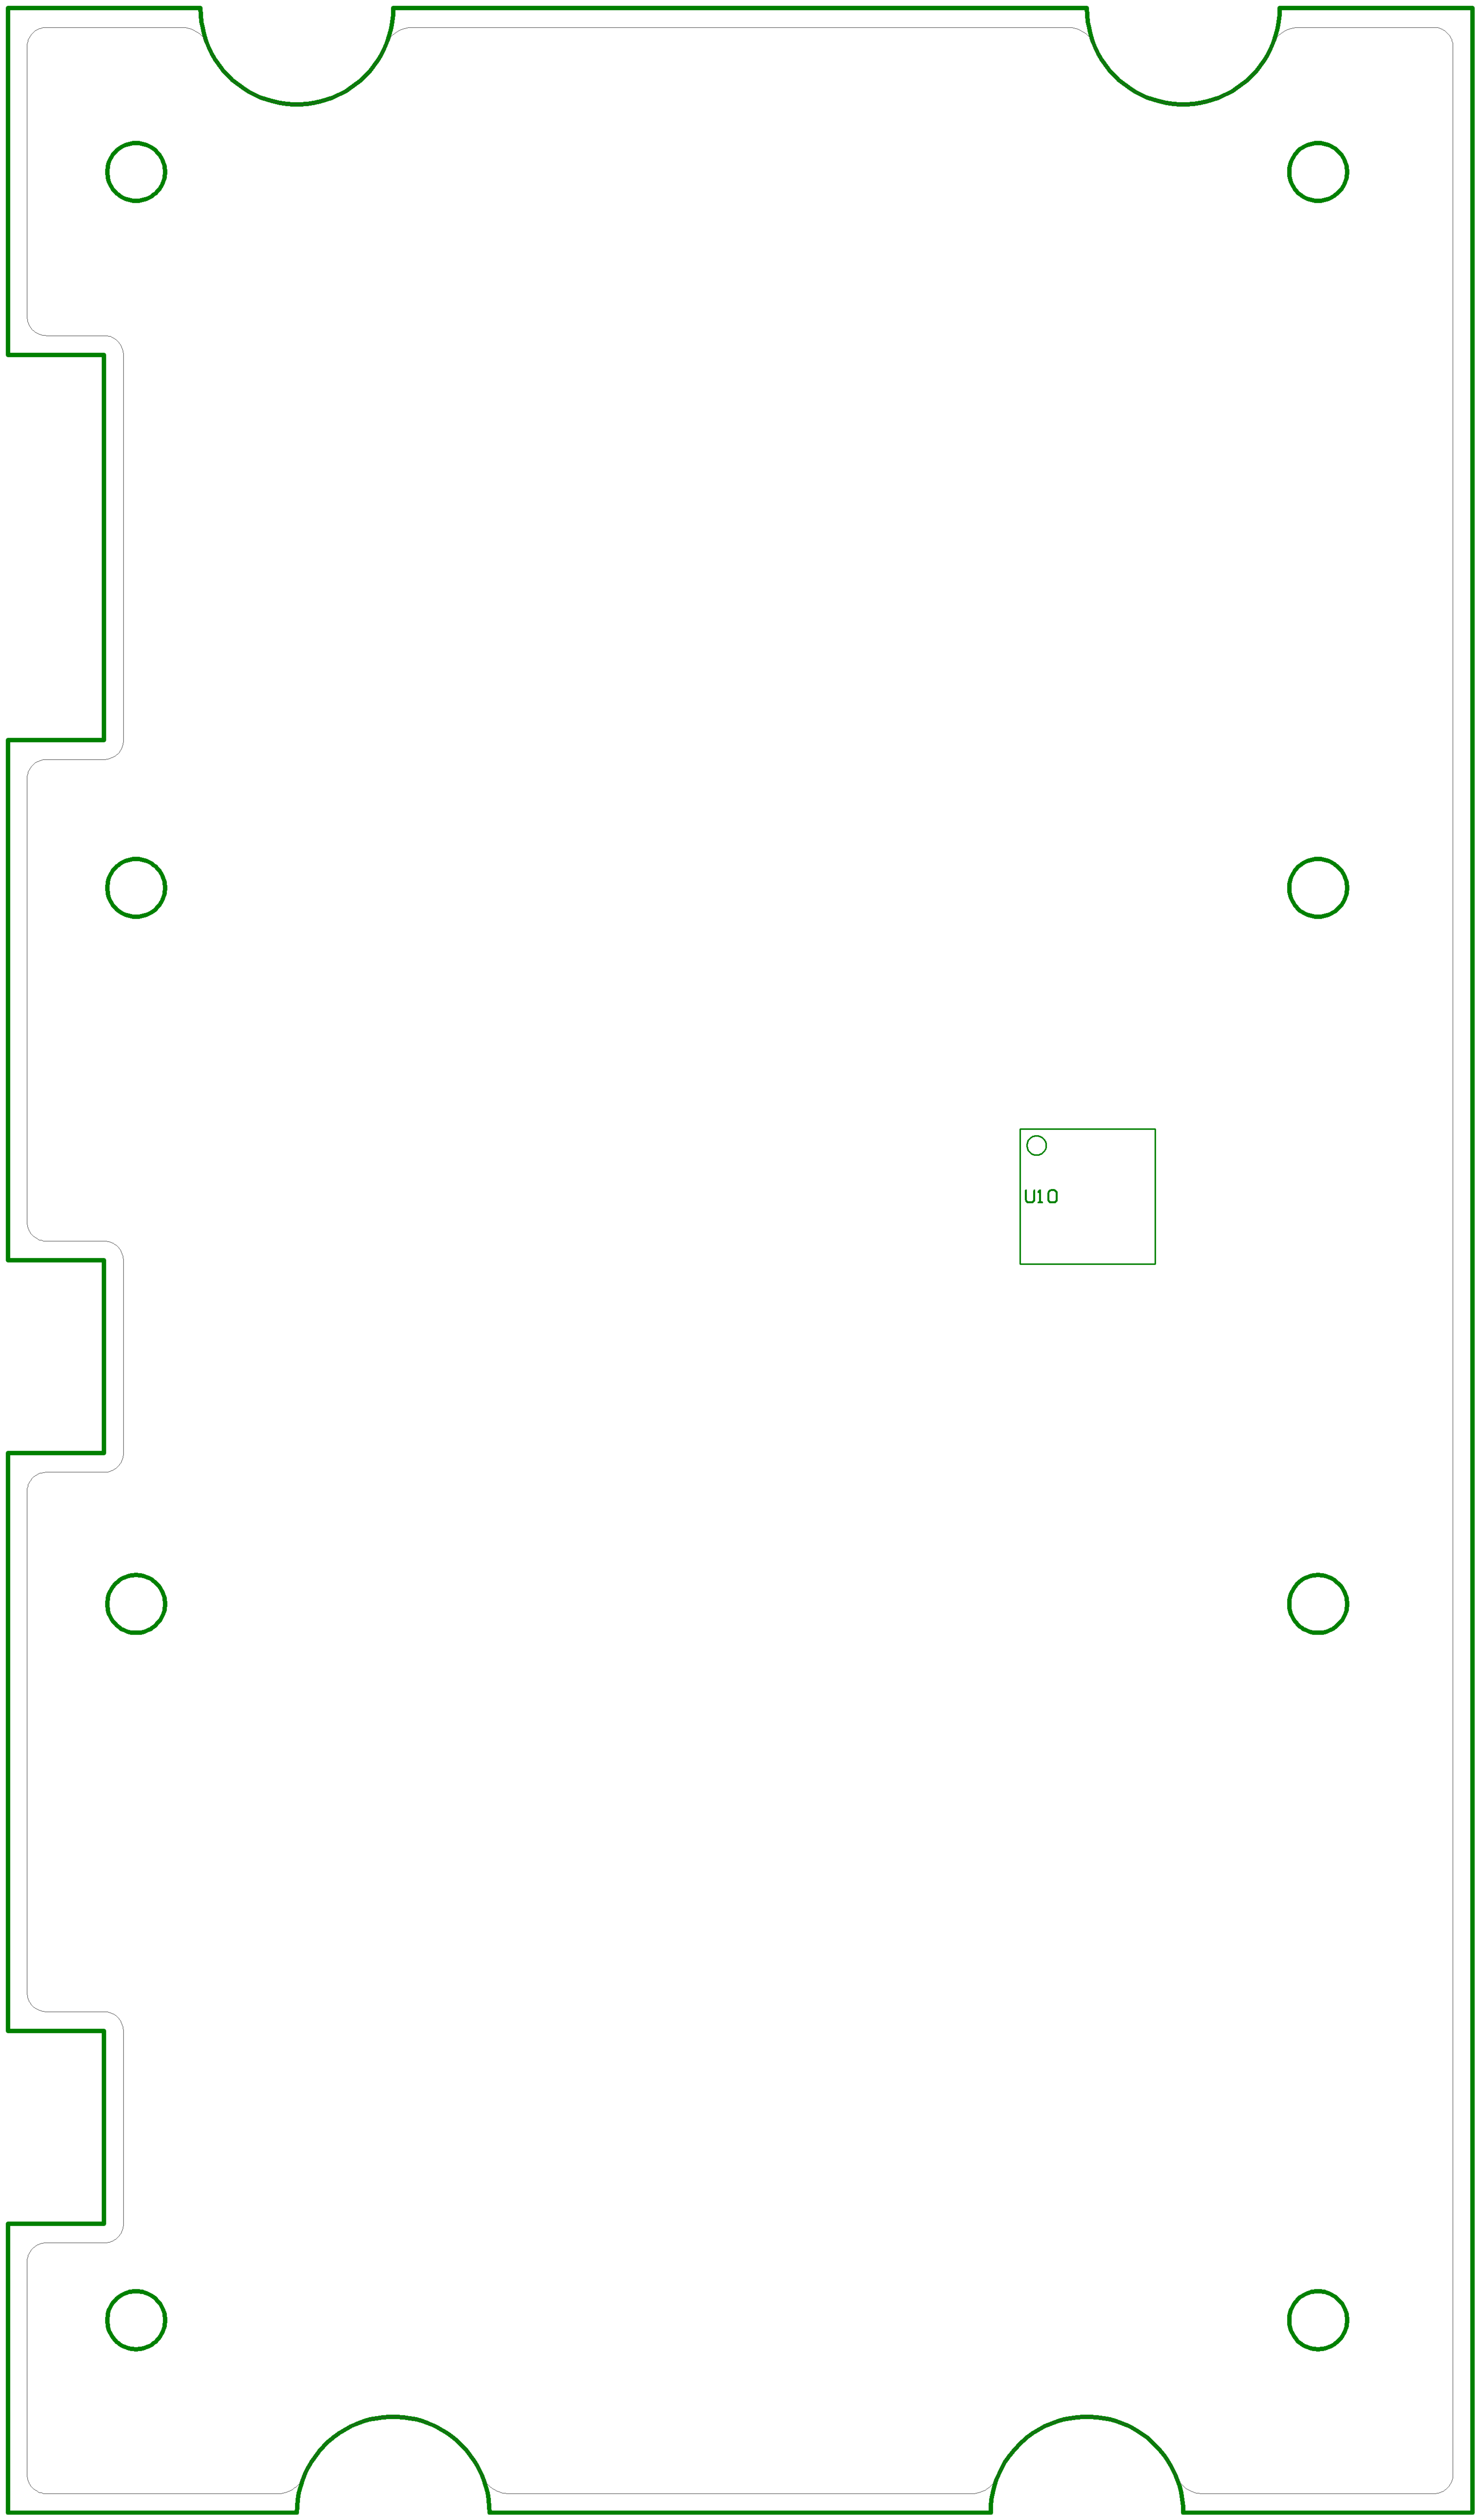
\includegraphics[width=\SmallSchematicWidth]{\Images/PCB/shape.eps}
    \caption{Board outlines}
    \label{img:board_shape}
\end{figure}

In green, and with right angles, there the exported shape from the mechanical conception.
We defined a bit smaller board shape than that, to ensure that the manufacturing tolerances
wont cause any issues, and to add some margin for some wires and so. This final board shape
is not clearly visible on the image, as it's drawn in grey and on a thin line.

There's a lot of mechanical support, by both screws and cuts to ensure the board can't be 
mounted backward. This is required to ensure the positing system has always the same 
reference position.

And, to finish, there some cutouts on the left side, to let more space for wirings. Thus, we
can easily make wires runs from the engines to the board without stressing them.

\subsection{Floorplan}
From all of theses settings, we can establish a first floorplan. As there is some cutouts for 
wires on the board, the position of some connectors / soldering pads need to be defined, to 
ensure the wire won't need to cross the board !
But there a lot of others elements with a defined position, theses includes : 

\begin{itemize}
    \item   Antennas and related ICs / passives 
    \item   Position of the accelerometers and IMU
    \item   Position of the screws.
\end{itemize}

\section{PCB Layout}
Now, we can start the layout process, in this order : 

\begin{itemize}
    \item   Place the remaining components on the board 
    \item   Route sensibles tracks.
    \item   Route the remaining tracks
\end{itemize}

\subsection{Component placement}
Our board is quite big for the components we needed to place. Thus, there is some empty spaces, 
which is not a bad thing.

This also mean that the placement of passives (which are, for most in the package size 0603) 
easier, since circuits are physically distants from others.

For each circuits, we always start with the decoupling capacitors, that need to be carrefully
placed near each power pins of the circuits. Then, we place the remaining passives that can 
be placed farther from the chip, for example pull up resistors.

This whole process was iterated two times. On the first pass, we globally place the components,
within 2 or 3 mm of their final position. Once the whole board was done, we've got a first idea 
of what the board was going to look, but there were a lot of smaller optimization that could be 
done. That's the goal of the second pass, we replace every component to a place that can be easier 
to route, aligned with the grid, and so.

\subsection{Pin swapping}
For the next step, we configured the "pin swapping" function on the schematic, to enable some pins 
to be swapped. This is possible due to the architecture of most recent microcontrollers, where all 
of the functions goes trough a pin matrix to assign to a pin, regardless of the peripheral. This 
gave us freedom on the crossing that can be deleted with it \footnote{
    This pin swapping method caused us some harm, because of an undoumented limitations : A 
    peripheral can't use, at the same time multiples pins from different ports. This required 
    us to re-route some part of the PCB.
}.
We created thus four groups of pins : 
\begin{itemize}
    \item   A digital group on the port where the function is pinned to the port 0.
    \item   Another digital group, for the port 1.
    \item   An analog input group.
    \item   A global group, for independant pins that can be used on any port.
\end{itemize}

Then, the ECAD tool enable us to automatically perform pin swapping to globally optimize the pins. 
Then, when routing, we can perform some precisions pin swaps if it make the layout easier.

\subsection{Layout}
When routing the connections, we've always got in mind the signal integrity issues than can come 
from mistakes at this point. 
Thus, we make sure that any fast signal \footnote{
    In fast, near every signal on the board can be qualified as fast, due to their rising and falling 
    edges. Nonetheless, for signals that enable or disable functions once in the flight, we assumed 
    that their behavior when switching aren't going to perturb the overall execution.
} is routed on top layers, or, by default with a ground plane near it. 

For every signals, if they need to "cross" a signal, on another layer, we ensured the crossing to be 
at a 90 degrees to reduce the crosstalk between them. In the same manner, we ensured that tracks that
are sensible won't couple inductively. This is done by separating them with enough space \footnote{A
    General rule of thumb is the 3W rule. Track center to the next center, there shall be 3 times the 
    width.}

For every track, we needed to route with a correct width, to ensure the current carying capacity will
large enough. Thus, for power tracks such as the 5V rail for the servo engines, or the engines starter,
we respectively used 1.5mm wide tracks. For the 3.3V rail, that power up all of the logic, the current
is smaller, a 1mm wide track is more than enough.

To be added, where there where a lot of pads of the same net to connect together, we used planes rather
than tracks. This greatly increase the current capacity of this area, for a null cost.

All of this work is shown on the images below, where we can see each layer, individually, with the 
standard Altium color code.

\begin{figure}[!hbt]
    \centering
    \begin{minipage}[c]{\SmallSchematicWidth}
        \centering
        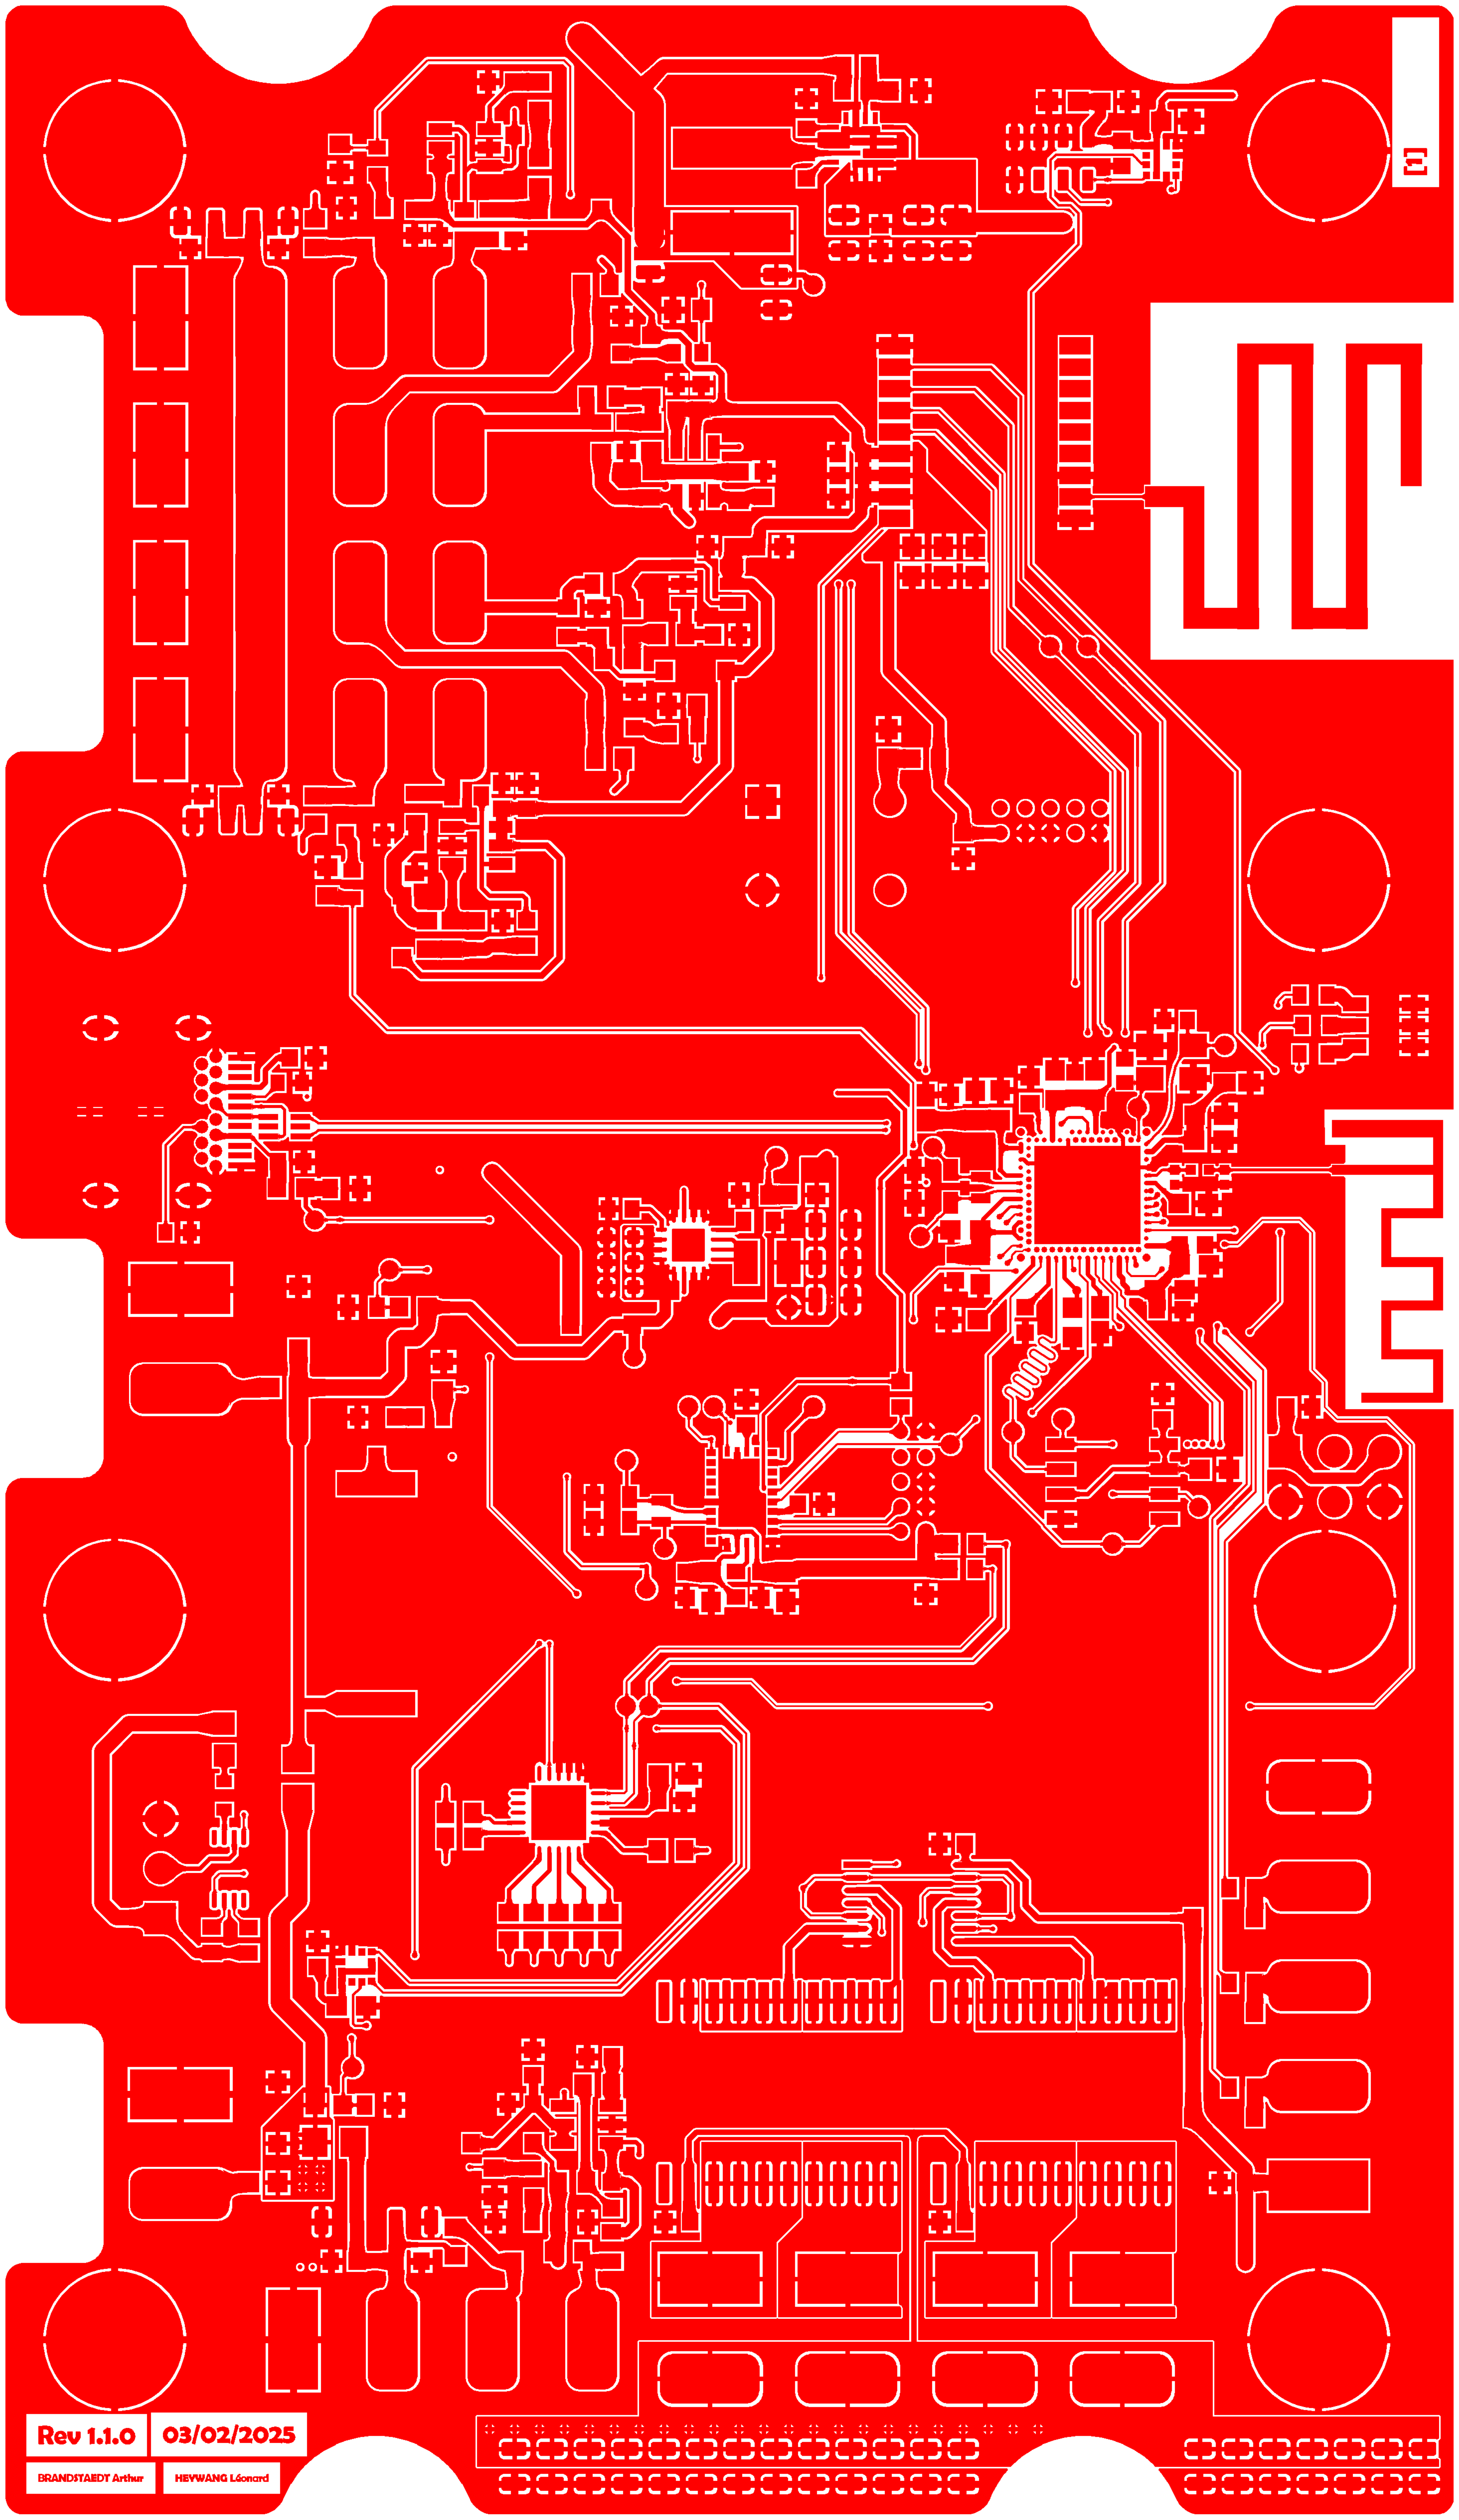
\includegraphics[width=\textwidth]{\Images/PCB/top.eps}
        \caption*{Copper layer (L1)}
    \end{minipage}%
    \hfill%
    \begin{minipage}[c]{\SmallSchematicWidth}
        \centering
        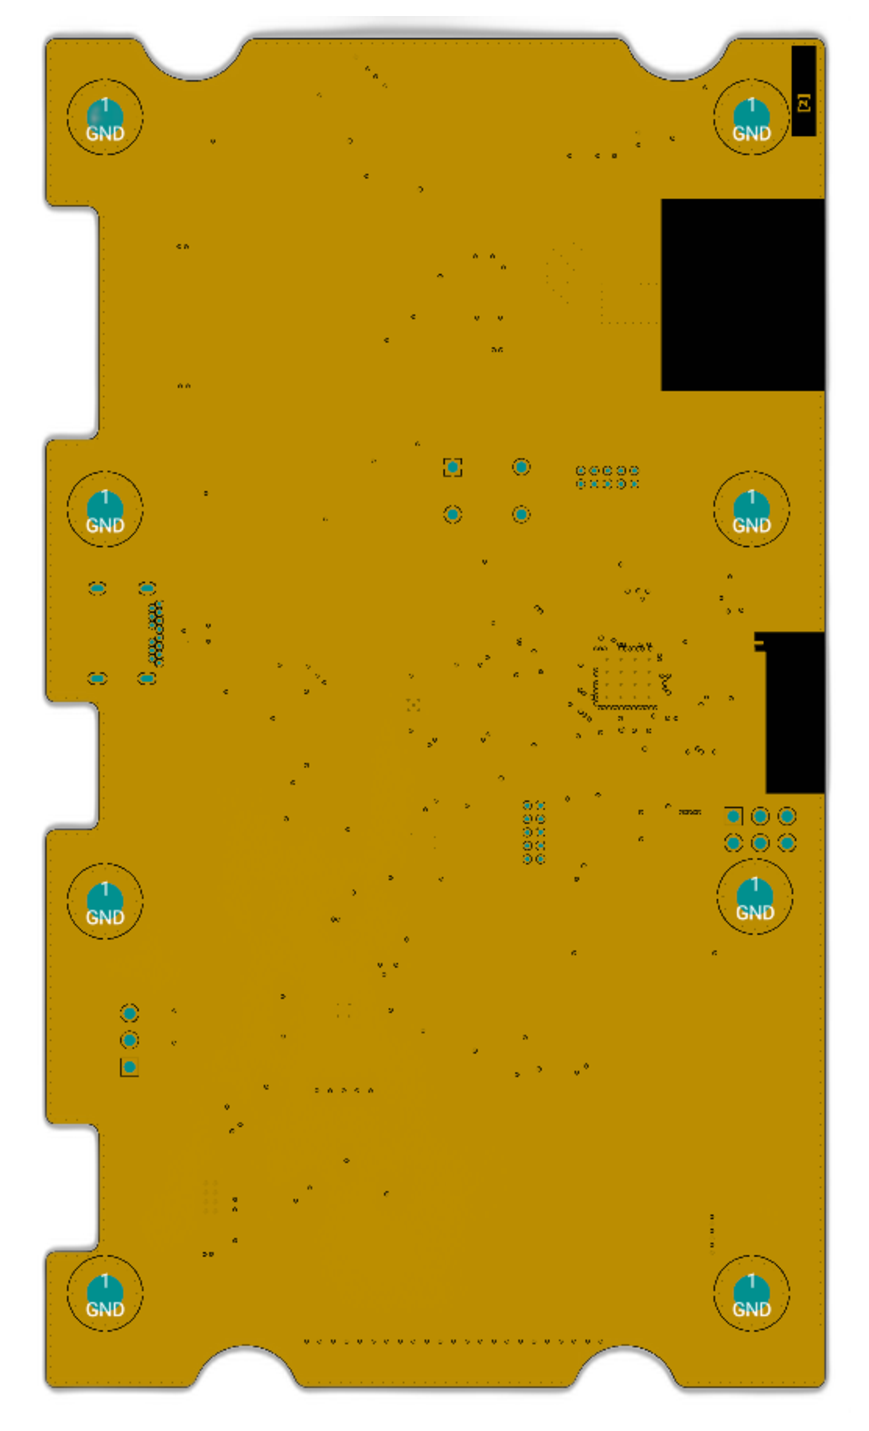
\includegraphics[width=\textwidth]{\Images/PCB/int1.eps}
        \caption*{Copper layer (L2)}
    \end{minipage}%
    \hfill%
    \begin{minipage}[c]{\SmallSchematicWidth}
        \centering
        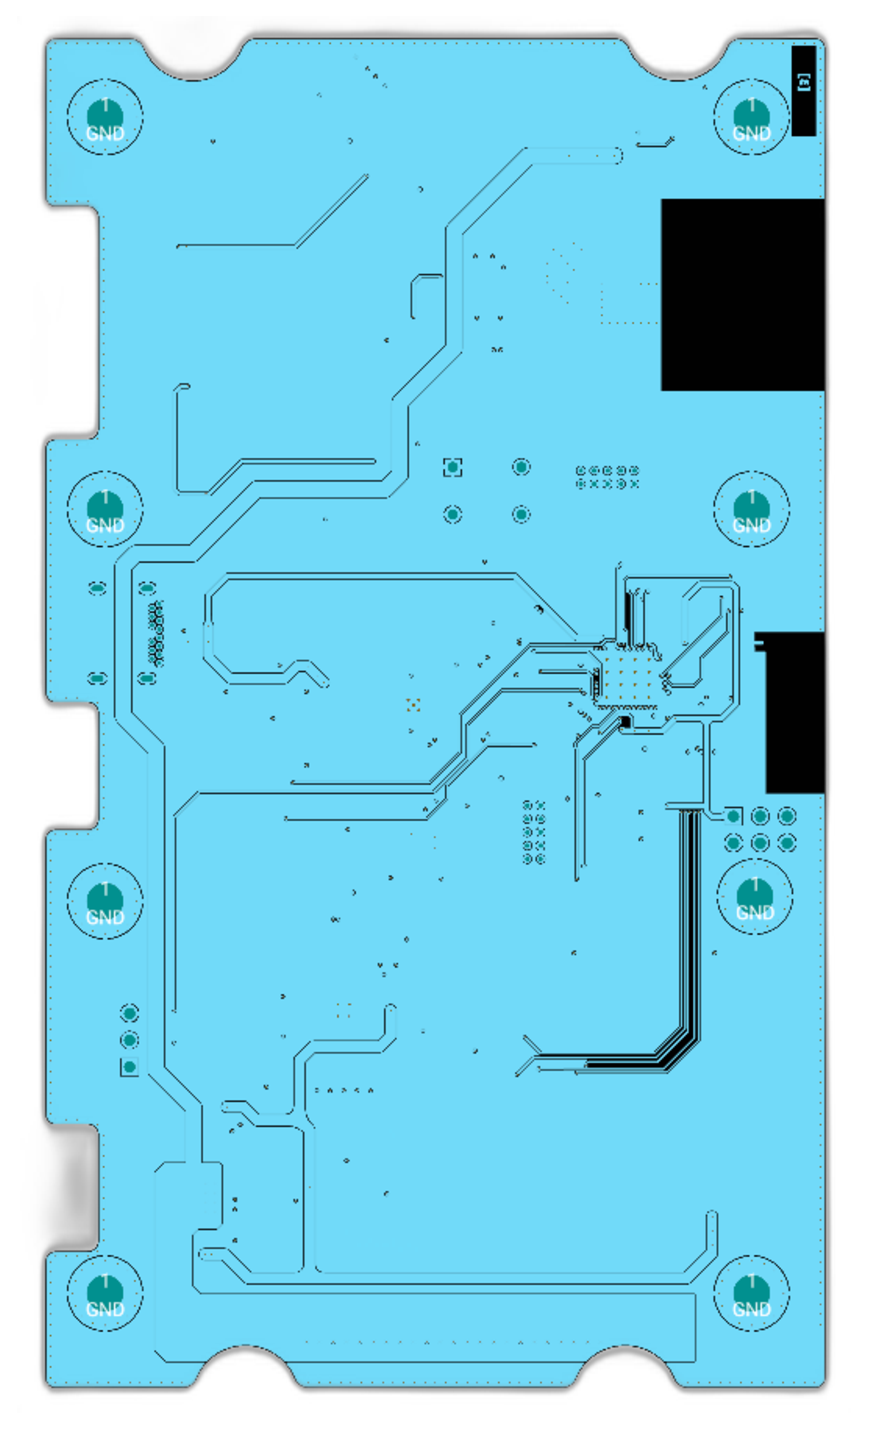
\includegraphics[width=\textwidth]{\Images/PCB/int2.eps}
        \caption*{Copper layer (L3)}
    \end{minipage}%
    \hfill%
    \begin{minipage}[c]{\SmallSchematicWidth}
        \centering
        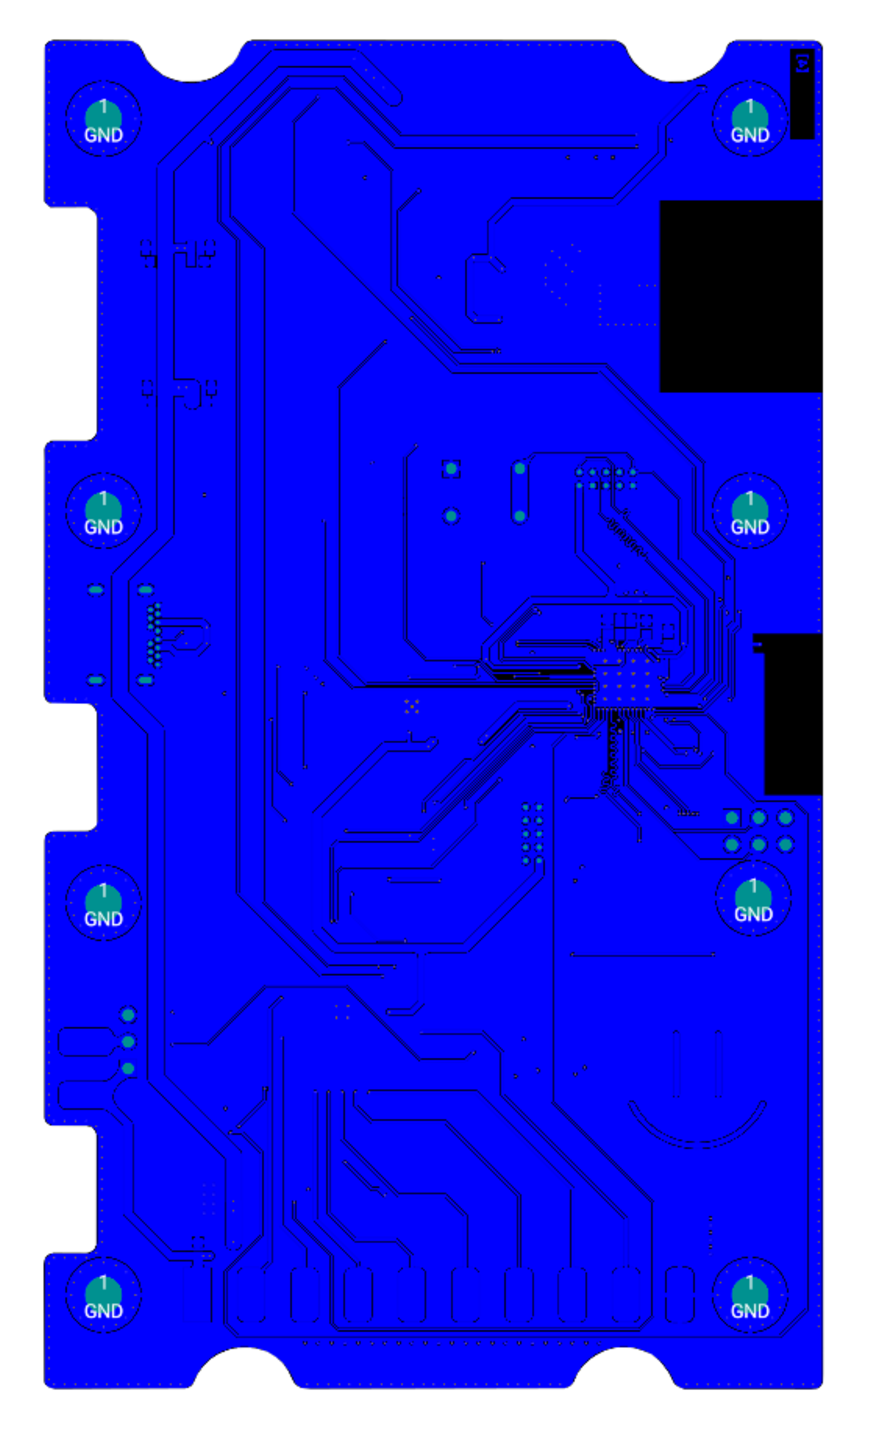
\includegraphics[width=\textwidth]{\Images/PCB/bot.eps}
        \caption*{Copper layer (L4)}
    \end{minipage}
    \label{img:layout}
    \caption{Copper layers on the PCB}
\end{figure}
\FloatBarrier

As explained before, we can cleary see that the first (L1) and last (L4) layers
are the most filled with tracks. The second layer (L2) is effectively empty of 
traces, to let the space for a whole ground plane, and, on the last layer there 
is the mix of both.
